\section{Resultados de rendimiento}
\label{sec:rendimiento}

% Fuentes: results/bench/secuencial_t1.csv (T14), results/bench/openmp.csv y
% results/bench/openmp_agregado.csv (T16/T18), results/bench/lita_i5-12400F/openmp.csv.
% Las cifras de esta sección se recalcularon desde esos CSV; si se regeneran, actualizar las tablas.

\subsection{Línea base secuencial}

En el equipo de referencia, con la configuración sintética de desarrollo ($p_{01} = 0{,}15$, $p_{11} = 0{,}60$, $\alpha = 0{,}7$, $\theta = \qty{9}{\milli\metre}$, $C = 6$~mm/día, $U = \qty{50}{\milli\metre}$, $D = 120$), $N = 2\times10^{7}$ temporadas y semilla \num{20261015}, la versión secuencial compilada en \codigo{Release} tarda $T_1 = \qty{59.70}{\second}$ con una desviación estándar de \qty{0.77}{\second} en cinco repeticiones. Equivale a \qty{2.985}{\micro\second} por temporada (unos \qty{25}{\nano\second} por día-escenario) y a un throughput de \num{3.35e5} escenarios por segundo. Todas las corridas obtuvieron $k = \num{2122915}$, es decir, $\phat = \num{0.10615}$ con intervalo de Wilson $[\num{0.10601};\ \num{0.10628}]$; la cifra solo verifica la salida, porque los parámetros no están calibrados.

El barrido OpenMP midió además su propia fila secuencial, $\qty{59.28}{\second}$ (desviación \qty{0.19}{\second}). Las métricas de la Tabla~\ref{tab:openmp} usan el $T_1$ de la medición oficial T14; con la fila del barrido, los speedups serían alrededor de un \num{0.7}\,\% menores.

\subsection{OpenMP en el equipo de referencia}

La Tabla~\ref{tab:openmp} y las Figuras~\ref{fig:openmp-tiempo}--\ref{fig:openmp-eficiencia} muestran el barrido de 2, 4, 8 y 16 hilos con tres \emph{schedules}: \codigo{static}, \codigo{dynamic} con bloque 1 (valor por defecto) y \codigo{dynamic} con bloque 64. Las 72 corridas OpenMP (12 puntos, cada uno con calentamiento y cinco repeticiones) dieron el mismo $k$ y el mismo histograma que la referencia secuencial (V1), y ningún punto está sobresuscrito en este equipo.

\begin{table}[!t]
\centering
\caption{OpenMP, $N = 2\times10^{7}$, $T_1 = \qty{59.70}{\second}$ (equipo de referencia)}
\label{tab:openmp}
\begin{tabular}{@{}lrrrrr@{}}
\toprule
\emph{Schedule} & $p$ & $T_p$ (s) & $S_p$ & $E_p$ & $e_p$ \\
\midrule
\multirow{4}{*}{\codigo{static}}
 & 2  & $29{,}96 \pm 0{,}81$ & 1,99  & 0,996 & 0,004 \\
 & 4  & $16{,}02 \pm 0{,}65$ & 3,73  & 0,932 & 0,024 \\
 & 8  & $10{,}01 \pm 0{,}34$ & 5,96  & 0,745 & 0,049 \\
 & 16 & $5{,}46 \pm 0{,}11$  & 10,94 & 0,684 & 0,031 \\
\midrule
\multirow{4}{*}{\codigo{dynamic:1}}
 & 2  & $32{,}13 \pm 1{,}24$ & 1,86  & 0,929 & 0,076 \\
 & 4  & $18{,}02 \pm 0{,}65$ & 3,31  & 0,828 & 0,069 \\
 & 8  & $9{,}97 \pm 0{,}30$  & 5,99  & 0,749 & 0,048 \\
 & 16 & $5{,}52 \pm 0{,}03$  & 10,81 & 0,676 & 0,032 \\
\midrule
\multirow{4}{*}{\codigo{dynamic:64}}
 & 2  & $29{,}82 \pm 0{,}22$ & 2,00  & 1,001 & $-0{,}001$ \\
 & 4  & $15{,}70 \pm 0{,}90$ & 3,80  & 0,951 & 0,017 \\
 & 8  & $9{,}46 \pm 0{,}11$  & 6,31  & 0,789 & 0,038 \\
 & 16 & $5{,}42 \pm 0{,}03$  & 11,01 & 0,688 & 0,030 \\
\bottomrule
\end{tabular}

\smallskip
\footnotesize $T_p$: media $\pm$ desviación estándar de cinco repeticiones. $e_p$: Karp--Flatt, Ec.~\eqref{eq:karpflatt}.
\end{table}

\begin{figure}[!t]
\centering
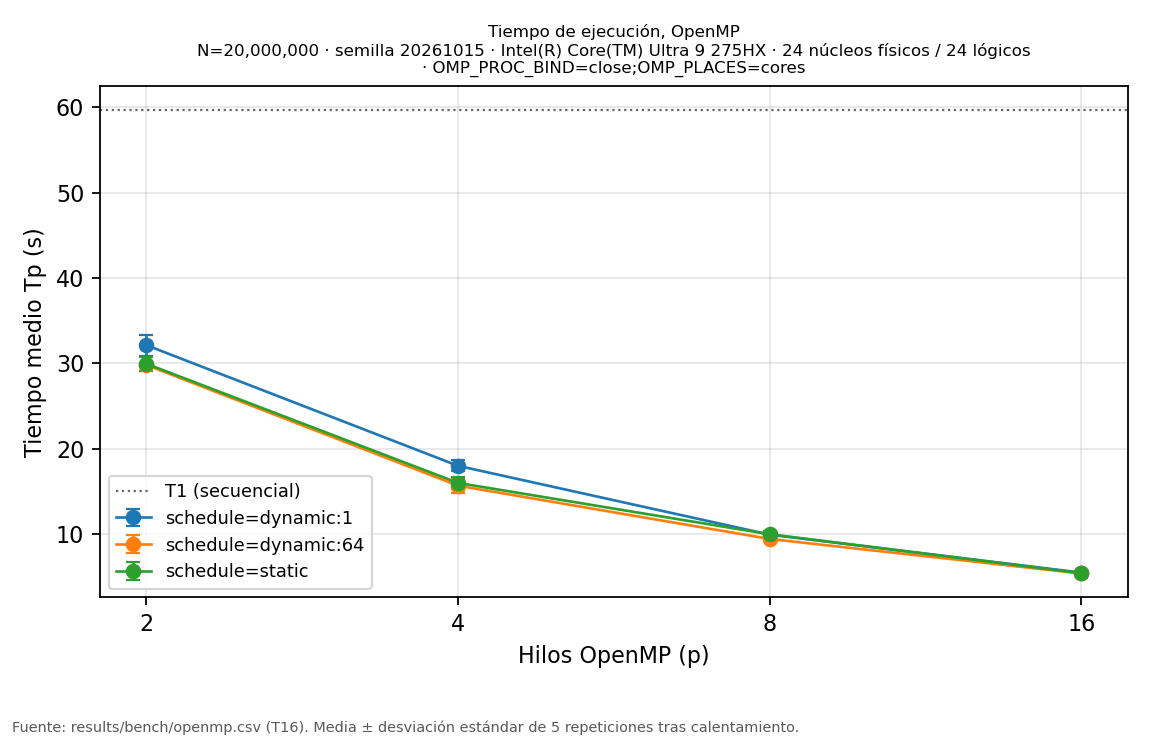
\includegraphics[width=\columnwidth]{openmp_tiempo.png}
\caption{Tiempo de pared OpenMP frente al número de hilos, con la referencia $T_1$; barras de error de una desviación estándar.}
\label{fig:openmp-tiempo}
\end{figure}

\begin{figure}[!t]
\centering
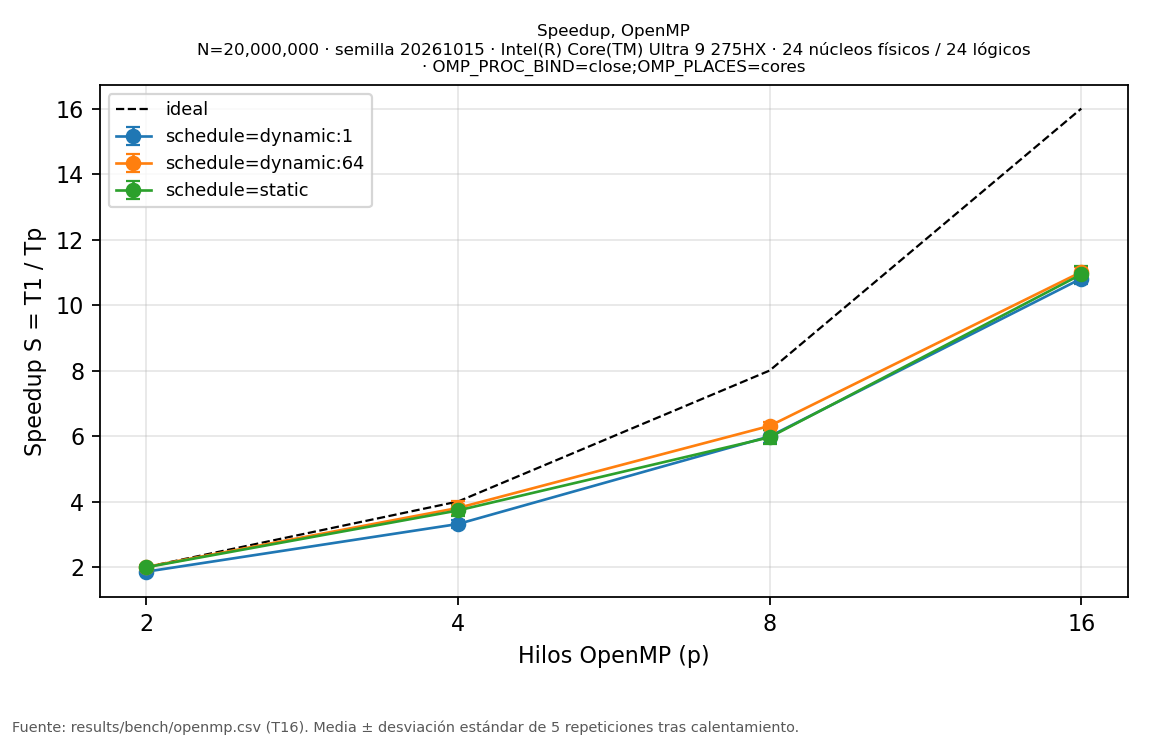
\includegraphics[width=\columnwidth]{openmp_speedup.png}
\caption{Speedup OpenMP por \emph{schedule}, con la recta ideal $S_p = p$.}
\label{fig:openmp-speedup}
\end{figure}

\begin{figure}[!t]
\centering
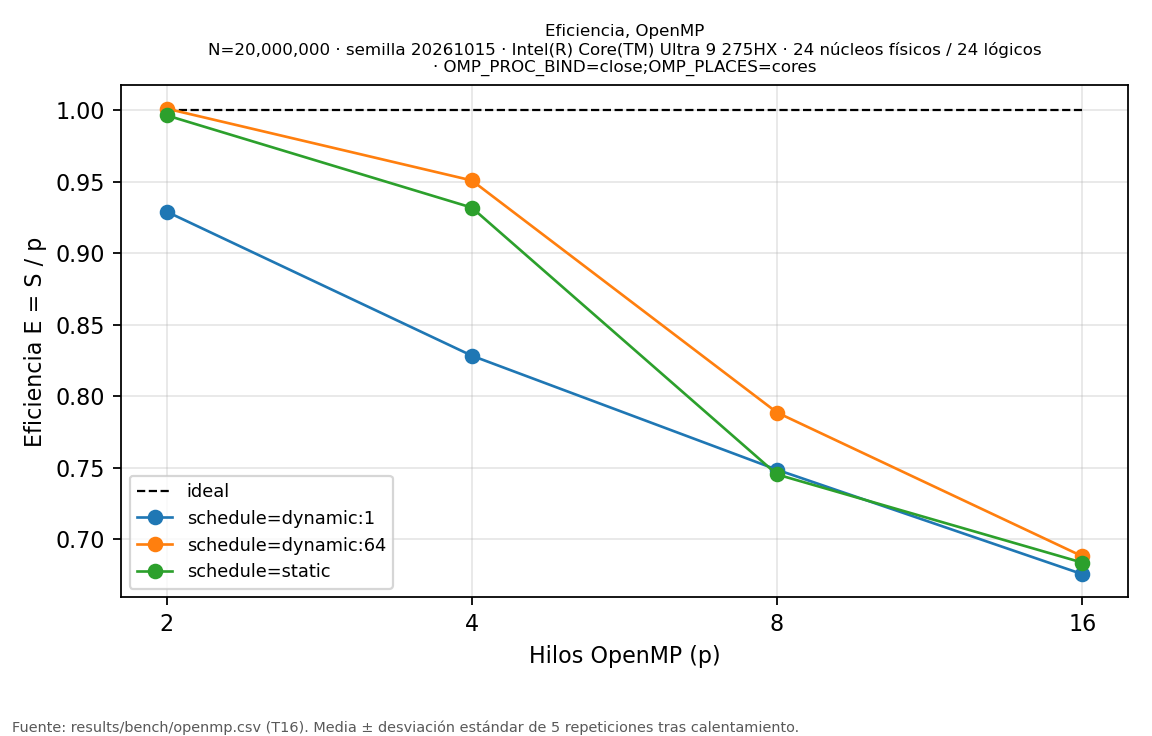
\includegraphics[width=\columnwidth]{openmp_eficiencia.png}
\caption{Eficiencia OpenMP por \emph{schedule}, con la referencia ideal $E_p = 1$.}
\label{fig:openmp-eficiencia}
\end{figure}

Con 2 y 4 hilos el speedup es casi lineal con \codigo{static} y \codigo{dynamic:64} ($E_p \ge 0{,}93$). Con 16 hilos los tres \emph{schedules} convergen a un speedup de 10,8--11,0 y una eficiencia de 0,68--0,69; el mejor punto es \codigo{dynamic:64}, con $S_{16} = 11{,}01$ y un throughput de \num{3.69e6} escenarios por segundo.

\codigo{dynamic:1} es el más lento con pocos hilos ($S_2 = 1{,}86$, $e_2 = 0{,}076$). Cada iteración dura unos \qty{3}{\micro\second}, por lo que repartir una iteración por solicitud hace que el costo de planificación de OpenMP sea apreciable; con bloques de 64 iteraciones ese costo se amortiza y el desequilibrio residual es despreciable, porque todas las temporadas tienen el mismo número de días. Con 8 hilos \codigo{dynamic:64} sigue siendo cerca de un 5\,\% más rápido que los otros dos; con 16 la diferencia entre \emph{schedules} baja a menos de un 2\,\%.

La fracción serial de Karp--Flatt no es monótona: crece hasta 8 hilos ($e_8 \approx 0{,}04$--$0{,}05$) y \emph{disminuye} con 16 ($e_{16} \approx 0{,}03$). Una fracción serial fija o una sobrecarga creciente de OpenMP harían que $e_p$ fuese constante o creciente. La explicación más consistente con el hardware es la heterogeneidad de núcleos: el equipo tiene 8 núcleos P, y a partir de 8 hilos parte del trabajo puede caer en núcleos E más lentos, de modo que $p$ hilos no equivalen a $p$ núcleos de igual capacidad. Por eso la pérdida de eficiencia entre 4 y 16 hilos no debe atribuirse solo a OpenMP. El bucle no comparte memoria ni sincroniza hilos dentro de la región, lo que es coherente con que el costo de la reducción final (un histograma de \qty{4}{\kilo\byte} por hilo) sea pequeño frente a segundos de cómputo.
% TODO-T33: confirmar la hipótesis P/E con una corrida de 8 hilos fijados a núcleos P (o con la medida por núcleo) antes de afirmarla en las conclusiones.

\subsection{OpenMP en el equipo 2}

Como contraste, el equipo~2 (6 núcleos físicos, 12 lógicos) midió $T_1 = \qty{71.01}{\second}$ (desviación \qty{0.57}{\second}) con la misma carga y obtuvo el mismo $k$. Con \codigo{static} logró speedups de 1,87, 3,39, 5,68 y 6,67 para 2, 4, 8 y 16 hilos, y con \codigo{dynamic:64}, de 1,89, 3,44, 5,96 y 7,32. Los puntos de 8 y 16 hilos están sobresuscritos ---16 hilos superan incluso los 12 lógicos---, por lo que la ganancia por encima de 6 hilos proviene de la ejecución simultánea en núcleos lógicos y no de núcleos adicionales; esos puntos no se usan para calcular eficiencia.

\subsection{MPI, híbrido y experimentos X1--X3}

% TODO-T33: insertar aquí, desde results/bench/mpi.csv, results/bench/hibrido.csv y los CSV de X1--X3:
%   (a) Tabla MPI E1 y E2 con 2/4/8/16 procesos: T_p ± desv., S_p, E_p, e_p, nodos y distribución por nodo.
%   (b) Tabla híbrido 2/4/8/16 núcleos totales con al menos dos factorizaciones P×T por presupuesto.
%   (c) X1 escalabilidad fuerte (N = 2×10^8) OpenMP vs. MPI vs. híbrido en el Swarm de tres equipos; figura de speedup y de Karp–Flatt.
%   (d) X2 escalabilidad débil (carga proporcional a p) con eficiencia de Gustafson.
%   (e) X3 barrido N = 10^6…10^9: tiempo y throughput frente a N; peso del costo fijo.
%   (f) X4 / T32: E1 frente a E2 con los mismos procesos en nodos heterogéneos (hipótesis H2).
%   Figuras esperadas: results/figures/mpi_*.png, hibrido_*.png, x1_*.png, x2_*.png, x3_*.png.
\textit{[Pendiente: resultados de MPI E1/E2, híbrido y experimentos X1--X4 en el clúster de tres equipos.]}
